\documentclass[12pt,a4paper,oneside]{report}
\usepackage[margin=0.8in]{geometry}
\usepackage{fontspec}
\setmainfont{Times New Roman}
\usepackage[none]{hyphenat} % Disable word breaking / hyphenation at the end of lines
\usepackage{graphicx}
\usepackage{array}
\usepackage{setspace}
\usepackage{listings}
\usepackage{xcolor}
\usepackage{cite}
\usepackage{caption}
\usepackage{enumitem} % Better control over lists spacing
\usepackage{amsmath} % Required for \text{} in equations

% Load hyperref for clickable TOC, citations, and links (all black)
\usepackage[colorlinks=true, linkcolor=black, citecolor=black, urlcolor=black]{hyperref}

% Customize citation style: numbers inside brackets in purple and italics
\renewcommand{\citeform}[1]{\textcolor{purple}{\itshape #1}}

% Set paragraph styles: no paragraph indentation and no paragraph skip
\setlength{\parindent}{0pt}
\setlength{\parskip}{0pt}
\emergencystretch=3em % Avoid text overflowing margins when hyphenation is disabled
\sloppy

% Set global line spacing to 1.5
\setstretch{1.5}

% Configure cell padding and alignment in tables
\renewcommand{\arraystretch}{1.1}
\newcolumntype{C}[1]{>{\centering\arraybackslash}m{#1}}

% Customize Chapter and Section Headings (RaggedRight, strict hierarchy, and Chapter X : Title format)
\usepackage{titlesec}
\titleformat{\chapter}[block]
  {\normalfont\fontsize{20}{24}\selectfont\bfseries\raggedright}
  {\chaptertitlename\ \thechapter\ :}{0.5em}{}
\titlespacing*{\chapter}{0pt}{0pt}{15pt}

\titleformat{\section}
  {\normalfont\fontsize{15}{18}\selectfont\bfseries\raggedright}
  {\thesection}{1em}{}
\titlespacing*{\section}{0pt}{10pt}{6pt}

\titleformat{\subsection}
  {\normalfont\fontsize{13}{16}\selectfont\bfseries\raggedright}
  {\thesubsection}{1em}{}
\titlespacing*{\subsection}{0pt}{8pt}{4pt}

% Configure Listings for Code Display
\definecolor{codegray}{rgb}{0.95,0.95,0.95}
\definecolor{codecomment}{rgb}{0.0,0.5,0.0}
\definecolor{codekeyword}{rgb}{0.0,0.0,0.8}
\definecolor{codestring}{rgb}{0.7,0.1,0.1}

\lstset{
  backgroundcolor=\color{codegray},
  commentstyle=\color{codecomment},
  keywordstyle=\color{codekeyword},
  stringstyle=\color{codestring},
  basicstyle=\ttfamily\fontsize{7.5}{9.0}\selectfont\linespread{1.0}\selectfont,
  breakatwhitespace=false,
  breaklines=true,
  captionpos=b,
  keepspaces=true,
  numbers=left,
  numberstyle=\tiny\color{gray},
  showspaces=false,
  showstringspaces=false,
  showtabs=false,
  tabsize=2,
  frame=single,
  rulecolor=\color{lightgray}
}

% Customize Contents title and depth (tocdepth=1 keeps it exactly on 1 page)
\renewcommand{\contentsname}{Contents}
\renewcommand{\bibname}{References}
\setcounter{tocdepth}{1}

\usepackage[titles]{tocloft}
\renewcommand{\cftchapfont}{\normalfont\bfseries\itshape}
\renewcommand{\cftchappagefont}{\normalfont\bfseries\itshape}

\begin{document}

% ==================== PAGE 1: TITLE PAGE ====================
\begin{titlepage}
\centering
\setstretch{1.3}
\vspace*{0.5in}
{\fontsize{28}{34}\selectfont\bfseries GESTURE CONTROLLED WIRELESS 4WD ROBOTIC CAR\par}
\vspace{0.8in}
{\fontsize{14}{18}\selectfont Mini Project Report Submitted in partial fulfilment of the requirements for the degree of Bachelor of Technology from Maulana Abul Kalam Azad University of Technology, West Bengal (formerly known as West Bengal University of Technology)\par}
\vspace{0.8in}
{\fontsize{14}{18}\selectfont By\par}
\vspace{0.2in}
{\fontsize{13}{17}\selectfont\bfseries
Sohan Ghosh (Roll No. 34900323050)\\
Sarupya Guha (Roll No. 34900323046)\\
Aushi Sarkar (Roll No. 34900323011)\\
Anupam Dutta (Roll No. 34900323003)\\
Joydip Das (Roll No. 34900323020)\par}
\vspace{0.5in}
{\fontsize{14}{18}\selectfont Under the Guidance of\par}
\vspace{0.2in}
{\fontsize{16}{20}\selectfont Project Supervisor: Dr. Gautam Das\par}
\vfill
{\fontsize{14}{18}\selectfont Department of Electronics and Communication Engineering \\ Cooch Behar Government Engineering College \\ Cooch Behar, West Bengal \\ 2026\par}
\vspace*{0.2in}
\end{titlepage}

\pagenumbering{roman}

% ==================== PAGE 2: ACKNOWLEDGEMENT & MEMBERS ====================
\newpage
\chapter*{Acknowledgement}
\addcontentsline{toc}{chapter}{Acknowledgement}
\vspace{0.1in}
First and foremost, I would like to express my deep sense of gratitude to our project supervisor, Dr. Gautam Das, and the Department of Electronics and Communication Engineering at Cooch Behar Government Engineering College for providing me with the opportunity to work on this interesting mini project. His constant guidance, technical feedback, and continuous support have been instrumental in the successful completion of this design and prototype realization.\par
\medskip
I am also very thankful to the laboratory instructors who provided the necessary electronic components, testing equipment, and workspace to construct and test the robotic vehicle. Finally, I would like to thank my family, friends, and peers for their constant encouragement and support throughout this work, which has given me valuable experience in hardware-software integration, sensor interfacing, and wireless communication protocols.\par

\vspace{0.2in}
\section*{Project Members}
\vspace{0.05in}
\begin{center}
\begin{tabular}{|C{4.5cm}|C{5.0cm}|C{5.0cm}|}
\hline
\textbf{Roll No.} & \textbf{Name of the Member} & \textbf{Signature of the Member} \\ \hline
34900323050 & Sohan Ghosh & \rule{0pt}{4ex} \\ \hline
34900323046 & Sarupya Guha & \rule{0pt}{4ex} \\ \hline
34900323011 & Aushi Sarkar & \rule{0pt}{4ex} \\ \hline
34900323003 & Anupam Dutta & \rule{0pt}{4ex} \\ \hline
34900323020 & Joydip Das & \rule{0pt}{4ex} \\ \hline
\end{tabular}
\end{center}
\clearpage

% ==================== PAGE 4: PUBLICATIONS AND ACRONYMS ====================
\chapter*{Publications and Acronyms}
\addcontentsline{toc}{chapter}{Publications and Acronyms}
\vspace{0.1in}
No academic research papers, patents, or conference presentations have been published from the research work and design findings presented in this mini project report so far. The system has been designed and implemented primarily as an educational prototype to fulfill the academic requirements of the Bachelor of Technology degree in Electronics and Communication Engineering.\par
\medskip
The following table lists the principal abbreviations, symbols, acronyms, and technical terms used in this mini project report, along with their definitions.\par
\vspace{0.1in}
\begin{center}
\fontsize{9.5}{11}\selectfont
\begin{tabular}{|C{3.0cm}|C{11.5cm}|}
\hline
\textbf{Acronym / Symbol} & \textbf{Description / Meaning} \\ \hline
ECE & Electronics and Communication Engineering \\ \hline
ESP-NOW & Low-latency, Connectionless Wi-Fi communication protocol by Espressif \\ \hline
MPU6050 & 6-axis Inertial Measurement Unit (Gyroscope and Accelerometer) \\ \hline
BO Motor & Brushed Outrunner DC motor with gear reduction \\ \hline
PWM & Pulse Width Modulation (used to control motor speed) \\ \hline
ADC & Analog-to-Digital Converter \\ \hline
I2C & Inter-Integrated Circuit serial communication protocol \\ \hline
GND & Electrical Common Ground \\ \hline
VCC & Voltage at the Common Collector (Positive Power Supply) \\ \hline
GPIO & General Purpose Input / Output pins \\ \hline
MEMS & Micro-Electro-Mechanical Systems \\ \hline
\end{tabular}
\vspace{0.05in}
\captionof{table}{List of Acronyms and Symbols}
\label{tab:acronyms}
\end{center}
\clearpage

% ==================== PAGE 5: TABLE OF CONTENTS ====================
\begin{singlespace}
\begingroup
\titleformat{\chapter}[block]
  {\normalfont\fontsize{22}{26}\selectfont\bfseries\itshape\raggedright}
  {}{0pt}{}
\tableofcontents
\endgroup
\end{singlespace}
\clearpage

% ==================== PAGE 6: LIST OF FIGURES & TABLES ====================
\begin{singlespace}
\chapter*{Lists of Figures and Tables}
\addcontentsline{toc}{chapter}{Lists of Figures and Tables}
\vspace{0.1in}
\begingroup
\renewcommand{\clearpage}{\relax}
\makeatletter
\renewcommand{\chapter}{\@ifstar{\@chapterstar}{\@chapternostar}}
\newcommand{\@chapterstar}[1]{%
  \vspace{10pt}%
  {\normalfont\fontsize{15}{18}\selectfont\bfseries\raggedright #1}\par%
  \nopagebreak\vspace{6.0pt}%
}
\newcommand{\@chapternostar}[2][]{%
  \vspace{10pt}%
  {\normalfont\fontsize{15}{18}\selectfont\bfseries\raggedright #2}\par%
  \nopagebreak\vspace{6.0pt}%
}
\makeatother
\listoffigures
\vspace{0.3in}
\listoftables
\endgroup
\end{singlespace}
\clearpage

% ==================== PAGE 7: ABSTRACT ====================
\chapter*{Abstract}
\vspace{0.2in}
This mini project presents the design, development, and physical implementation of a wireless, gesture-controlled 4-wheel drive (4WD) robotic vehicle. The system utilizes dual ESP32 microcontrollers to establish a low-latency, connectionless peer-to-peer communication link using Espressif's ESP-NOW protocol. The transmitter glove consists of an ESP32 board interfaced with an MPU6050 6-axis inertial measurement unit. As the user tilts their hand, the sensor measures changes in gravitational acceleration and angular velocity, and translates these movements into Pitch and Roll orientation parameters. The transmitter ESP32 processes these angles and transmits the packets wirelessly to the receiver ESP32 on the robot chassis.\par
\medskip
At the receiving end, the receiver ESP32 decodes the incoming data packets and controls two L298N dual H-Bridge motor drivers. These drivers regulate the direction and speed of four 200 RPM dual shaft BO motors mounted on a 4WD chassis. The report details the core working principle of the MPU6050, the exact electrical connections for both the transmitter and receiver circuits, and the software methodology for fetching MAC addresses to establish secure communication. The physical prototype has been fully assembled, calibrated, and tested. The experimental results show that the gesture-controlled vehicle moves forward, backward, left, right, and stops reliably, validating its use in warehouse automation, search-and-rescue, and assistive interfaces.\par
\clearpage

\pagenumbering{arabic}

% ==================== PAGE 8: CHAPTER 1: INTRODUCTION ====================
\chapter{Introduction}
\section{Project Overview}
Robotics plays an increasingly important role in modern industries, warehouse logistics, and everyday life. Traditional methods of controlling robotic vehicles, such as joysticks, keyboards, or mobile applications, require manual dexterity and physical contact. Over the past few years, the development of natural human-machine interfaces has become a major research focus \cite{hmi_ref}. Gesture-based control represents a significant advancement, allowing humans to interact with machines using intuitive physical movements. By using wearable motion sensors, a user can control a robotic platform simply by tilting their hand, eliminating the need for complex control pads. Kinematic modeling of mobile robots forms the basis of design optimization and autonomous navigation \cite{robotics_ref}.\par
\medskip
This project focuses on building a gesture-controlled 4-wheel drive robot car using the ESP32 microcontroller and the MPU6050 motion sensor. The design translates the natural tilt of a user's wrist into control commands. If the hand tilts forward, the car moves forward; if it tilts backward, the car reverses; and left or right tilts steer the car in those directions. Wireless communication modules transmit these commands from the hand-worn controller to the mobile chassis. This system is highly useful for hazardous environments, search-and-rescue operations, and assisting individuals with limited mobility who find traditional controllers difficult to use.

\section{Review of Previous Works}
In early designs, wired connections linked accelerometers directly to the robot chassis, which restricted the range of movement. Later implementations introduced wireless modules like infrared (IR) and Bluetooth. However, IR requires line-of-sight and Bluetooth has range limitations and pairing delays. Radio Frequency (RF) modules operating at 433 MHz became popular due to their low cost and simple interfaces. The primary challenge with basic RF modules is their susceptibility to electromagnetic noise and lack of built-in data verification \cite{motor_ref}.\par
\medskip
Recently, advanced microcontrollers like the ESP32 have introduced high-speed, low-latency protocols \cite{sensor1}. Espressif's ESP-NOW protocol operates on the 2.4 GHz band and allows peer-to-peer communication without a router, reducing latency to a few milliseconds \cite{espnow_ref}. Similarly, modern digital sensors like the MPU6050 combine a 3-axis accelerometer and a 3-axis gyroscope on a single chip \cite{imu_main}. It communicates via I2C and filters out mechanical vibrations using an onboard Digital Motion Processor. This project focuses on building a robust prototype utilizing the ESP32/MPU6050/ESP-NOW architecture, demonstrating how connectionless wireless configurations improve mobile robot steering.

\section{Objective and Motivation}
The primary objective of this project is to design, construct, and evaluate a wireless, gesture-controlled 4WD robot car that responds in real time to wrist gestures. The motivation is to create intuitive control interfaces. Gesture control mimics natural physical actions, making it easy for untrained users to operate. Furthermore, in industrial warehouses or search-and-rescue scenarios, hands-free gesture controls can improve operational safety and speed. By testing different configurations, we aim to build a reliable prototype that balances range, response time, and battery life.

\section{Scope of Present Work}
The present work details the design and physical assembly of a gesture-controlled robotic car. The scope includes:
\begin{enumerate}[noitemsep,topsep=2pt,parsep=0pt,partopsep=0pt]
    \item Interfacing the MPU6050 sensor with the transmitter ESP32 to read tilt \cite{imu_main}.
    \item Calibrating threshold angles to define stable movement states.
    \item Implementing wireless transfer via the connectionless ESP-NOW protocol \cite{espnow_ref}.
    \item Integrating two L298N motor drivers with four 200 RPM dual shaft BO motors.
    \item Design analysis of an upgraded ESP32/ESP-NOW circuit topology using Mecanum wheels for diagonal and spot rotation movements.
\end{enumerate}
To compare these systems, Table \ref{tab:comparison} outlines the technical specs of the ESP32 design.\par
\vspace{0.05in}
\begin{center}
\fontsize{9.0}{10.5}\selectfont
\begin{tabular}{|C{3.2cm}|C{11.2cm}|}
\hline
\textbf{Feature} & \textbf{ESP32 Wireless Setup} \\ \hline
Microcontrollers & Two ESP32 Dev Boards (Transmitter \& Receiver) \\ \hline
Sensor Type & MPU6050 (6-Axis Digital I2C Gyro/Accelerometer) \\ \hline
Wireless Protocol & ESP-NOW (2.4 GHz Peer-to-Peer, Connectionless) \\ \hline
Chassis Motors & Four 200 RPM Dual Shaft BO Geared Motors \\ \hline
Micro-controller Interfacing & Direct GPIO lines to Dual L298N drivers \\ \hline
Typical Latency & 5 -- 15 ms \\ \hline
Noise Immunity & High (CRC check, frequency hopping, direct pairing) \\ \hline
\end{tabular}
\vspace{0.05in}
\captionof{table}{Project System Specifications}
\label{tab:comparison}
\end{center}
\clearpage

% ==================== PAGE 10: CHAPTER 2: HARDWARE ARCHITECTURE ====================
\chapter{Hardware Architecture and Component Details}
\section{Microcontrollers}
Microcontrollers process sensor inputs and coordinate motor drivers. This project uses the ESP32 Development Board for both the transmitter and receiver \cite{sensor1}. The ESP32 is a 32-bit dual-core processor running at 240 MHz. It has built-in Wi-Fi and Bluetooth, allowing board-to-board communication via the low-latency ESP-NOW protocol. It has 520 KB of SRAM, 4 MB of Flash memory, and a wide array of GPIO pins that support I2C, SPI, UART, and hardware PWM, making it highly suited for real-time robotic control applications.

\section{Sensors}
The sensor detects hand tilt by measuring acceleration along its axes. The MPU6050 6-axis IMU is utilized in this design \cite{imu_main}. The MPU6050 combines a 3-axis accelerometer and a 3-axis gyroscope on a single silicon die. The accelerometer measures the projection of gravitational acceleration along the X, Y, and Z axes, which allows the microcontroller to compute static tilt angles (Pitch and Roll). The gyroscope measures the angular rate of rotation around these axes, which is crucial for tracking dynamic wrist rotation (Yaw). It communicates with the ESP32 over an I2C serial bus, ensuring high noise immunity. Figure \ref{fig:comp_tx} shows the transmitter components.
\vspace{0.1in}
\begin{center}
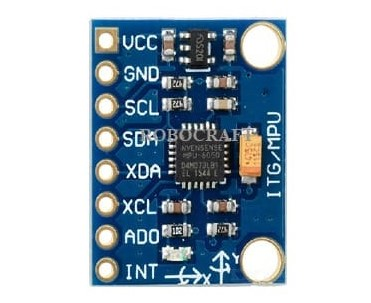
\includegraphics[width=0.5\textwidth,height=5.2cm,keepaspectratio=true]{images/comp-img1.jpeg}
\captionof{figure}{Transmitter Hardware Assembly showing ESP32, MPU6050, and Wearable Assembly}
\label{fig:comp_tx}
\end{center}

\section{Wireless Communication Protocol}
The wireless link transmits motion commands from the glove to the robot chassis. Espressif's ESP-NOW protocol is utilized in STA (Station) mode to achieve high-performance direct wireless transfer \cite{espnow_ref}. Unlike traditional Wi-Fi which requires connection to a router and introduces handshaking delays, ESP-NOW uses a connectionless, peer-to-peer packet transmission mechanism. It operates on the 2.4 GHz band and allows the transmitter to send packets directly to the receiver's MAC address. This reduces latency to under 10 milliseconds, making it ideal for real-time mobile chassis steering.

\section{Motor Drivers and Actuators}
The motors require more current than microcontroller pins can supply.
\begin{enumerate}[noitemsep,topsep=2pt,parsep=0pt,partopsep=0pt]
    \item \textbf{L298N Motor Driver}: We use two L298N H-Bridge drivers \cite{motor_ref}. The L298N can drive four DC motors in pairs, handling up to 2A per channel. It regulates speed via PWM and direction via digital logic pins. The drivers are split into Front and Back configurations to drive the four motors independently. The dual H-bridge topology is highly effective for controlling the speed and direction of DC geared motors independently. Figure \ref{fig:comp_rx} shows the receiver module and L298N driver.
    \item \textbf{Actuators}: The actuators are four 200 RPM dual shaft BO (Battery Operated) geared motors. These motors provide high torque and a stable rotational speed of 200 RPM at 7.4V. The dual shafts allow encoder mounting or mechanical alignment.
\end{enumerate}
\vspace{0.05in}
\begin{center}
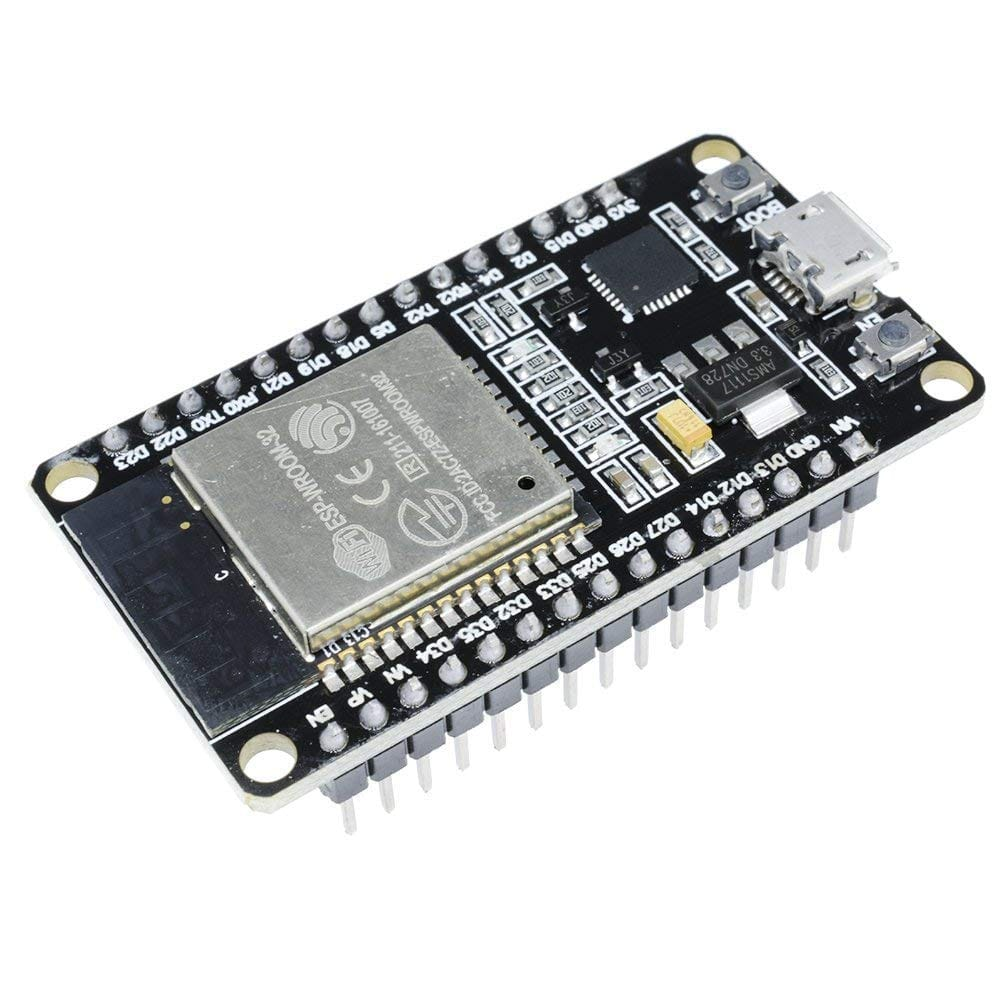
\includegraphics[width=0.5\textwidth,height=5.2cm,keepaspectratio=true]{images/comp-img2.jpeg}
\captionof{figure}{Receiver Hardware Assembly with Dual L298N Motor Drivers and ESP32 Receiver Module}
\label{fig:comp_rx}
\end{center}

\section{Power Source and Accessories}
Two 18650 Lithium-Ion cells in series provide a 7.4V pack to power the motor drivers. The driver's onboard 5V regulator provides regulated power to the microcontrollers, establishing a clean common ground system.
\clearpage

% ==================== PAGE 12: CHAPTER 3: SYSTEM DESIGN ====================
\chapter{System Design and Circuit Integration}
\section{Transmitter Schematic and Connections}
The transmitter module reads hand tilt and sends movement codes wirelessly. The MPU6050 accelerometer detects changes in gravity along the X and Y axes as the hand tilts. The transmitter ESP32 communicates with the MPU6050 via the hardware I2C bus. The connections are wired as follows: VCC of MPU6050 is connected to the 3.3V pin of the ESP32, GND is connected to the common ground (GND), SCL is connected to GPIO 22, and SDA is connected to GPIO 21. The code compares these readings against calibrated thresholds to determine if the hand is tilted forward, backward, left, or right. Figure \ref{fig:block_diag} shows the overall system block diagram.\par
\vspace{0.15in}
\begin{center}
\makebox[\textwidth][c]{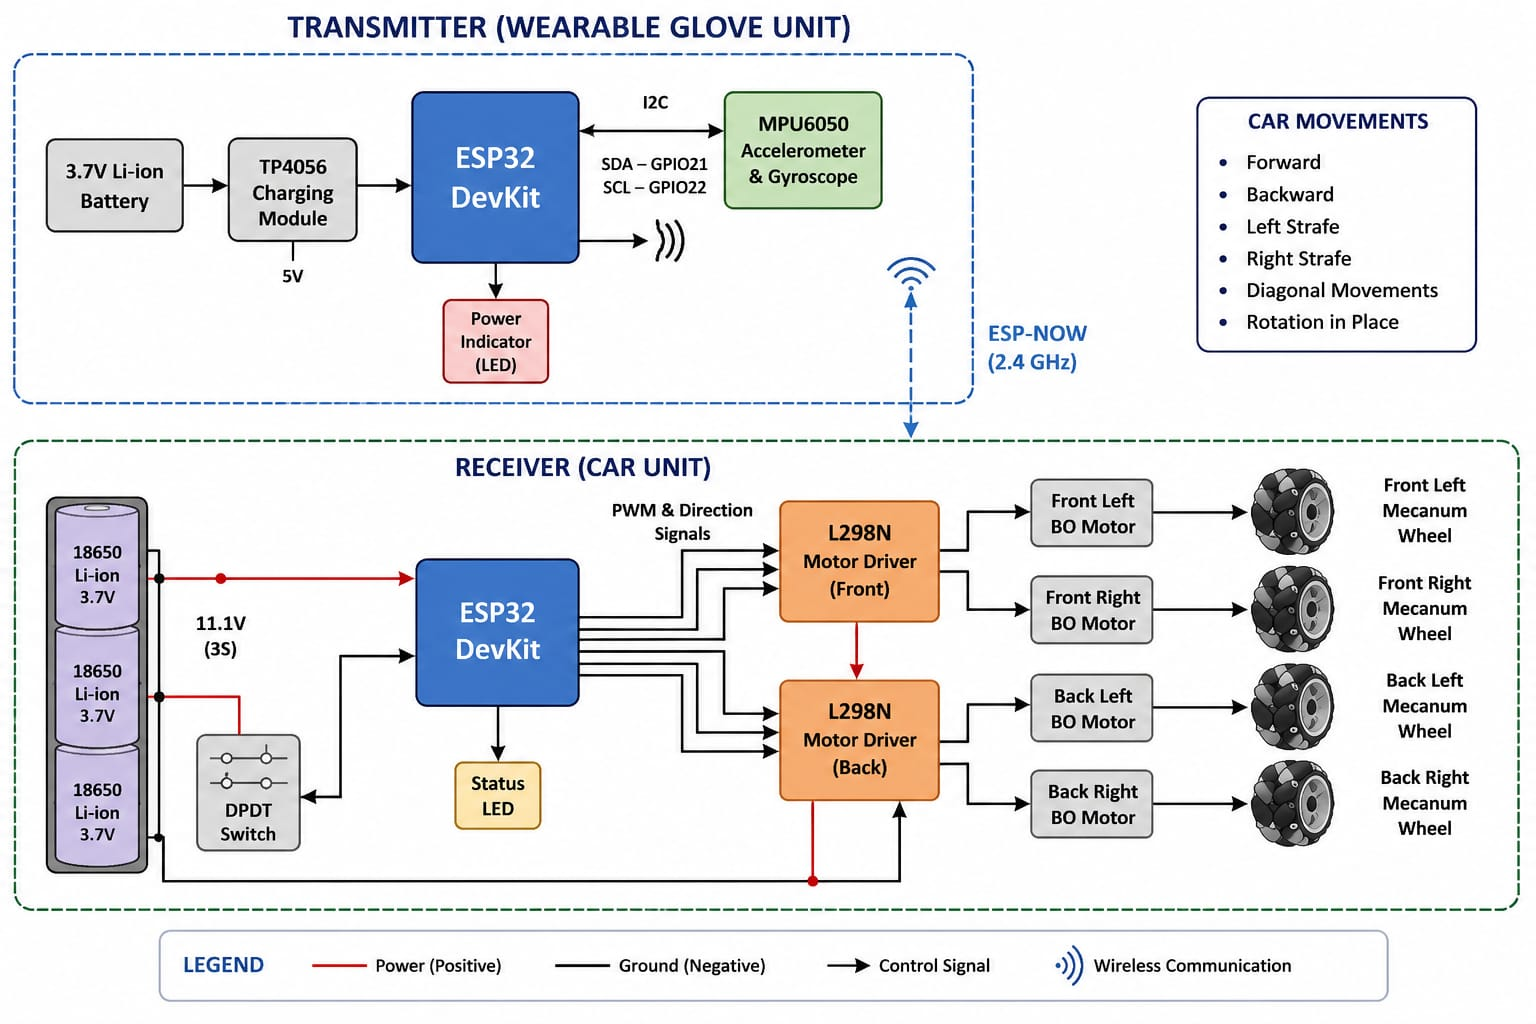
\includegraphics[width=1.1\textwidth,height=10.2cm,keepaspectratio=true]{images/block-diagram.png}}
\captionof{figure}{Gesture-Controlled Car System Block Diagram showing the ESP32 transmitter and receiver architecture}
\label{fig:block_diag}
\end{center}
\clearpage

\begin{center}
\begin{tabular}{|C{4.0cm}|C{4.0cm}|C{6.0cm}|}
\hline
\textbf{MPU6050 Pin} & \textbf{ESP32 GPIO} & \textbf{Function} \\ \hline
VCC & 3.3V & Power Supply (3.3V) \\ \hline
GND & GND & Electrical Ground \\ \hline
SCL & GPIO 22 & I2C Serial Clock \\ \hline
SDA & GPIO 21 & I2C Serial Data \\ \hline
\end{tabular}
\vspace{0.05in}
\captionof{table}{MPU6050 to Transmitter ESP32 Connections}
\label{tab:mpu_conn}
\end{center}

\section{Receiver Schematic and Connections}
The receiver chassis decodes the ESP-NOW signals and drives the motors. The receiver ESP32 decodes the signals and determines the movement state. It then controls two L298N motor drivers. Since this is a 4-wheel drive car, the motors are paired: the front-left and back-left motors are driven together, and the front-right and back-right motors are driven together. Figure \ref{fig:l298n_bb} shows the wiring connections between the ESP32 and the L298N motor driver. The pins are configured as shown in Tables \ref{tab:pins_front} and \ref{tab:pins_back}.\par
\vspace{0.15in}
\begin{center}
\makebox[\textwidth][c]{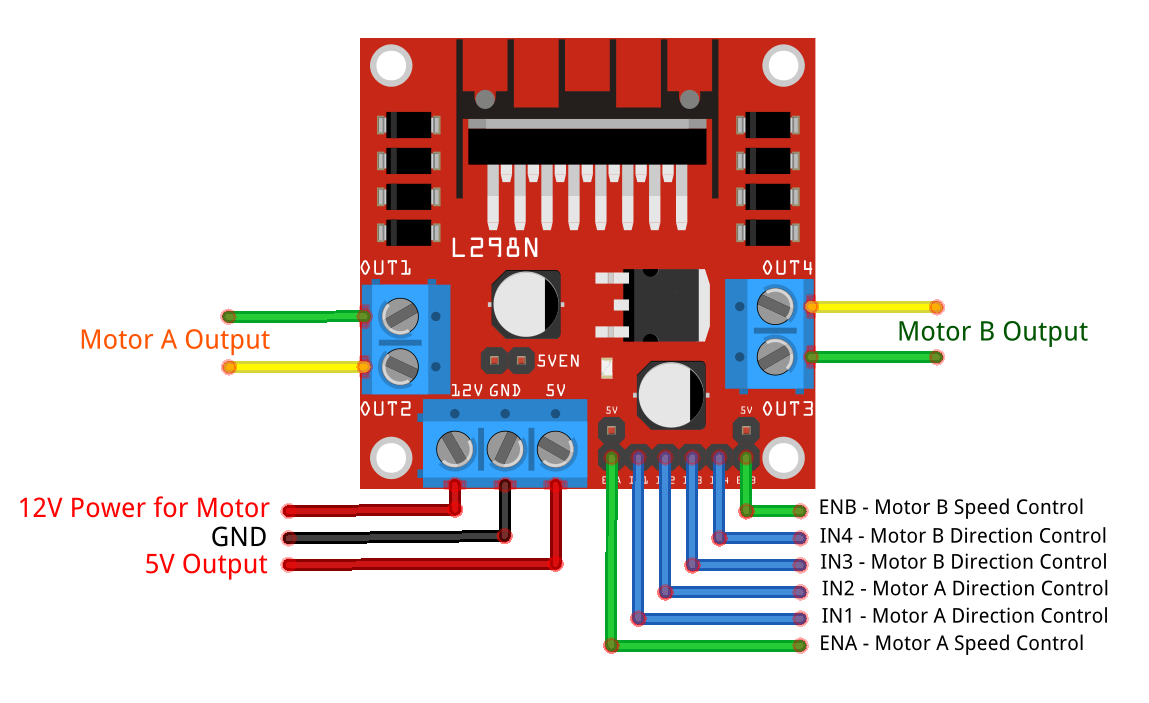
\includegraphics[width=1.05\textwidth,height=9.2cm,keepaspectratio=true]{images/l298n_motordriver_pinout_bb.png}}
\captionof{figure}{Fritzing Wiring Diagram showing L298N Motor Driver connections to ESP32 Receiver}
\label{fig:l298n_bb}
\end{center}

\section{ESP32 GPIO Pin Connections}
In the primary ESP32 gesture-controlled vehicle architecture, the pins are mapped directly to ensure high-performance, independent 4-wheel motor drive control. Tables \ref{tab:pins_front} and \ref{tab:pins_back} show the pin mappings for the Front and Back L298N motor drivers respectively.\par
\vspace{0.1in}
\begin{center}
\begin{minipage}{0.48\textwidth}
  \centering
  \fontsize{9.5}{11}\selectfont
  \begin{tabular}{|C{2.3cm}|C{2.0cm}|C{2.0cm}|}
  \hline
  \textbf{ESP32 GPIO} & \textbf{L298N} & \textbf{Function} \\ \hline
  GPIO 32 & ENA & PWM Speed \\ \hline
  GPIO 33 & IN1 & FR Motor Dir 1 \\ \hline
  GPIO 25 & IN2 & FR Motor Dir 2 \\ \hline
  GPIO 26 & IN3 & FL Motor Dir 1 \\ \hline
  GPIO 27 & IN4 & FL Motor Dir 2 \\ \hline
  GPIO 14 & ENB & PWM Speed \\ \hline
  \end{tabular}
  \vspace{0.05in}
  \captionof{table}{Front L298N ESP32 Pins}
  \label{tab:pins_front}
\end{minipage}
\hfill
\begin{minipage}{0.48\textwidth}
  \centering
  \fontsize{9.5}{11}\selectfont
  \begin{tabular}{|C{2.3cm}|C{2.0cm}|C{2.0cm}|}
  \hline
  \textbf{ESP32 GPIO} & \textbf{L298N} & \textbf{Function} \\ \hline
  GPIO 22 & ENA & PWM Speed \\ \hline
  GPIO 16 & IN1 & RR Motor Dir 1 \\ \hline
  GPIO 17 & IN2 & RR Motor Dir 2 \\ \hline
  GPIO 18 & IN3 & RL Motor Dir 1 \\ \hline
  GPIO 19 & IN4 & RL Motor Dir 2 \\ \hline
  GPIO 23 & ENB & PWM Speed \\ \hline
  \end{tabular}
  \vspace{0.05in}
  \captionof{table}{Back L298N ESP32 Pins}
  \label{tab:pins_back}
\end{minipage}
\end{center}

\section{Mecanum Wheel Kinematics and Movement Matrix}
The ESP32 vehicle chassis is equipped with four Mecanum wheels, which contain rollers mounted at 45-degree angles to the wheel perimeter. This roller configuration creates directional force vectors that enable holonomic motion \cite{robotics_ref}. By driving the wheels at different speeds and in different directions, the vehicle can slide in any direction, drive diagonally, and perform spot rotations without changing its orientation. Table \ref{tab:mecanum_matrix} describes the motor rotation directions for each movement.\par
\vspace{0.1in}
\begin{center}
\fontsize{9.0}{11}\selectfont
\begin{tabular}{|C{2.7cm}|C{2.7cm}|C{2.7cm}|C{2.7cm}|C{2.7cm}|}
\hline
\textbf{Robot Action} & \textbf{Front Left} & \textbf{Front Right} & \textbf{Back Left} & \textbf{Back Right} \\ \hline
Move Forward & Forward & Forward & Forward & Forward \\ \hline
Move Backward & Reverse & Reverse & Reverse & Reverse \\ \hline
Lateral Left & Reverse & Forward & Forward & Reverse \\ \hline
Lateral Right & Forward & Reverse & Reverse & Forward \\ \hline
Diagonal F-Left & Stop & Forward & Forward & Stop \\ \hline
Diagonal F-Right & Forward & Stop & Stop & Forward \\ \hline
Rotate Left & Reverse & Forward & Reverse & Forward \\ \hline
Rotate Right & Forward & Reverse & Forward & Reverse \\ \hline
Stop & Stop & Stop & Stop & Stop \\ \hline
\end{tabular}
\vspace{0.05in}
\captionof{table}{Mecanum Wheel Movement Matrix}
\label{tab:mecanum_matrix}
\end{center}
\newpage
\section{Power Scheme and Common Grounding}
To prevent voltage spikes, electromagnetic interference (EMI), and transient voltage drops caused by the high current draw of the DC geared motors from resetting or damaging the sensitive ESP32 microcontrollers, a robust split power delivery configuration is implemented in this robotic car.\par
\medskip
The power source consists of a high-capacity 7.4V Lithium-Ion battery pack using two 18650 cells connected in series. The positive terminal of this battery pack supplies raw 7.4V directly to the motor power input pins ($V_{MS}$ or $12V$ input terminal) of the dual L298N motor driver boards. This ensures that the heavy currents required by the four BO motors during start-up, acceleration, and stalling do not pass through the microcontroller's power lanes.\par
\medskip
The L298N driver boards feature an onboard 5V regulator (specifically the LM7805 or similar linear regulator chip). This regulator steps down the 7.4V input to a stable, regulated 5V output, which is fed into the $5V$ or $VIN$ pins of the ESP32 boards. To ensure stable operation, 100\textmu{}F electrolytic capacitors are placed in parallel with the power lines to smooth out voltage fluctuations, and 0.1\textmu{}F ceramic capacitors are added across the motor terminals to suppress high-frequency electrical noise generated by the motor brushes.\par
\medskip
A critical design rule in this circuit integration is establishing a unified common ground. Connecting the negative terminals (GND) of the battery pack, the ESP32 microcontroller, and both L298N motor drivers is absolutely essential. Without a shared common ground reference, the control PWM signals sent from the ESP32 GPIO pins to the motor driver inputs (IN1--IN4, ENA, ENB) would lack a stable return path, causing erratic motor behaviors or communication failure.\par

% ==================== PAGE 15: CHAPTER 4: SOFTWARE IMPLEMENTATION ====================
\chapter{Software Implementation and Control Algorithms}
\section{Development Environment}
\label{sec:dev_env}
The control firmware was developed using the Arduino IDE 2.x and written in C++ with standard microcontroller libraries:
\begin{itemize}[noitemsep,topsep=2pt,parsep=0pt,partopsep=0pt]
    \item \textbf{Wire.h}: Enables I2C communication between the ESP32 and the MPU6050 sensor.
    \item \textbf{MPU6050.h} and \textbf{I2Cdev.h}: Interfaces with the MPU6050 IMU to retrieve orientation data.
    \item \textbf{esp\_now.h} and \textbf{WiFi.h}: Operates the ESP-NOW protocol on the ESP32's built-in 2.4 GHz transceiver.
\end{itemize}

\section{Retrieving the ESP32 MAC Address}
To establish peer-to-peer communication using ESP-NOW, the transmitter ESP32 must know the exact physical Media Access Control (MAC) address of the receiver ESP32 \cite{espnow_ref}. The MAC address is a unique 48-bit identifier assigned to the network interface card during manufacturing. To retrieve this MAC address, a simple initialization sketch is uploaded to the receiver board. This code initializes the Wi-Fi stack in station mode and prints the MAC address to the Serial Monitor. Listing 4.1 shows the retrieval code.
\begin{lstlisting}[language=C++, caption={ESP32 MAC Address Fetching Sketch}]
#include <WiFi.h>

void setup() {
  Serial.begin(115200);
  WiFi.mode(WIFI_STA); // Set Wi-Fi to Station mode
  delay(1000);
  Serial.print("ESP32 Board MAC Address: ");
  Serial.println(WiFi.macAddress()); // Output MAC address
}

void loop() {
  // Empty loop as MAC address is only fetched once
}
\end{lstlisting}

\section{Transmitter Firmware Logic}
The transmitter ESP32 reads raw acceleration values along the X, Y, and Z axes from the MPU6050 register. The code calculates Pitch and Roll using trigonometric functions:
\begin{equation}
\text{Pitch} = \text{atan2}(-a_x, \text{sqrt}(a_y^2 + a_z^2)) \times \frac{180}{\pi}
\end{equation}
\begin{equation}
\text{Roll} = \text{atan2}(a_y, a_z) \times \frac{180}{\pi}
\end{equation}
These calculated angles can be filtered using complementary filtering to remove high-frequency mechanical vibration noise \cite{imu_filter}. The processed angles are then scaled using the `map()` function between 0 and 254 and packaged into a structural format. The struct is then sent via ESP-NOW to the receiver MAC address.

\section{Receiver Firmware Logic}
The receiver ESP32 registers a callback function that triggers whenever a packet is received via ESP-NOW. It extracts the pitch and roll values, then decodes the gesture orientation based on calibrated threshold boundaries:
\begin{itemize}[noitemsep,topsep=2pt,parsep=0pt,partopsep=0pt]
    \item \textbf{Tilted Forward} (Pitch $<$ 100): Rotates all wheels forward.
    \item \textbf{Tilted Backward} (Pitch $>$ 150): Rotates all wheels backward.
    \item \textbf{Tilted Left} (Roll $<$ 100): Slides the car left by reversing FL/RR and driving FR/RL forward.
    \item \textbf{Tilted Right} (Roll $>$ 150): Slides the car right by driving FL/RR forward and reversing FR/RL.
    \item \textbf{Diagonal Movements}: Triggers when both pitch and roll cross their thresholds simultaneously.
\end{itemize}

\section{Control Code Listings}
The listings below detail the source codes for the transmitter and receiver ESP32-based ESP-NOW system.
\begin{lstlisting}[language=C++, caption={ESP32 Transmitter Code (ESP-NOW with MPU6050 Pitch/Roll mapping)}]
// Transmitter
#include <esp_now.h>
#include <WiFi.h>
#include <Wire.h>
#include <MPU6050_tockn.h>

MPU6050 mpu(Wire);

typedef struct { char command; } PacketData;
PacketData data;

uint8_t receiverMAC[] = {0x20, 0xE7, 0xC8, 0x7C, 0xBE, 0xD4};

char getCommand(float pitch, float roll) {
  bool fwd = pitch > 20, back = pitch < -20;
  bool left = roll < -20, right = roll > 20;

  if (roll < -45) return 'A';               // rotate left
  if (roll > 45)  return 'D';               // rotate right
  if (fwd && left)  return 'Q';             // forward-left
  if (fwd && right) return 'E';             // forward-right
  if (back && left)  return 'Z';            // backward-left
  if (back && right) return 'C';            // backward-right
  if (fwd)  return 'F';                     // forward
  if (back) return 'B';                     // backward
  if (left)  return 'L';                    // strafe left
  if (right) return 'R';                    // strafe right
  return 'S';                               // stop
}

void setup() {
  Serial.begin(115200);
  WiFi.mode(WIFI_STA);
  Wire.begin(21, 22);
  mpu.begin();
  delay(1000);
  Serial.println("Keep MPU Flat");
  mpu.calcGyroOffsets(true);

  if (esp_now_init() != ESP_OK) {
    Serial.println("ESP NOW INIT FAILED");
    return;
  }

  esp_now_peer_info_t peerInfo = {};
  memcpy(peerInfo.peer_addr, receiverMAC, 6);
  peerInfo.channel = 0;
  peerInfo.encrypt = false;
  esp_now_add_peer(&peerInfo);

  Serial.println("READY");
}

void loop() {
  mpu.update();
  data.command = getCommand(mpu.getAngleX(), mpu.getAngleY());

  esp_now_send(receiverMAC, (uint8_t*)&data, sizeof(data));

  Serial.print("CMD: ");
  Serial.println(data.command);
  delay(20);
}
\end{lstlisting}
\begin{lstlisting}[language=C++, caption={ESP32 Receiver Code (ESP-NOW Mecanum Control)}]
// Listing 4.3 - ESP32 Receiver Code
#include <esp_now.h>
#include <WiFi.h>
#include <vector>

enum Movement {
  STOP, FORWARD, BACKWARD, LEFT, RIGHT,
  FORWARD_LEFT, FORWARD_RIGHT, BACKWARD_LEFT, BACKWARD_RIGHT,
  TURN_LEFT, TURN_RIGHT
};

enum MotorIndex { BR, BL, FR, FL };  // back-right, back-left, front-right, front-left

struct MOTOR_PINS { int pinIN1, pinIN2, pinEn; };

std::vector<MOTOR_PINS> motorPins = {
  {26, 18, 32},  // BACK RIGHT
  {19, 23, 15},  // BACK LEFT
  {13, 12, 33},  // FRONT RIGHT
  {14, 27, 25}   // FRONT LEFT
};

const int PWMFreq = 1000;
const int PWMResolution = 8;
const int targetSpeed = 220;
int currentSpeed = 0;

#define SIGNAL_TIMEOUT 1000
unsigned long lastRecvTime = 0;

typedef struct { char command; } PacketData;
PacketData receiverData;

// Per-movement motor speed multipliers: {FR, BR, FL, BL} as fractions of spd (-1, 0, 1)
const int movementTable[11][4] = {
  /* STOP           */ {0, 0, 0, 0},
  /* FORWARD        */ {1, 1, 1, 1},
  /* BACKWARD       */ {-1, -1, -1, -1},
  /* LEFT           */ {1, -1, -1, 1},
  /* RIGHT          */ {-1, 1, 1, -1},
  /* FORWARD_LEFT   */ {1, 0, 0, 1},
  /* FORWARD_RIGHT  */ {0, 1, 1, 0},
  /* BACKWARD_LEFT  */ {0, -1, -1, 0},
  /* BACKWARD_RIGHT */ {-1, 0, 0, -1},
  /* TURN_LEFT      */ {1, 1, -1, -1},
  /* TURN_RIGHT     */ {-1, -1, 1, 1},
};

int smooth(int speed) {
  if (currentSpeed < speed) currentSpeed = min(currentSpeed + 15, speed);
  else if (currentSpeed > speed) currentSpeed = max(currentSpeed - 15, speed);
  return currentSpeed;
}

void rotateMotor(int motorNumber, int motorSpeed) {
  digitalWrite(motorPins[motorNumber].pinIN1, motorSpeed > 0 ? HIGH : LOW);
  digitalWrite(motorPins[motorNumber].pinIN2, motorSpeed < 0 ? HIGH : LOW);
  ledcWrite(motorPins[motorNumber].pinEn, abs(motorSpeed));
}

void processCarMovement(int movement) {
  int spd = (movement == STOP) ? 0 : smooth(targetSpeed);
  if (movement == STOP) currentSpeed = 0;

  const int* m = movementTable[movement];
  rotateMotor(FR, m[0] * spd);
  rotateMotor(BR, m[1] * spd);
  rotateMotor(FL, m[2] * spd);
  rotateMotor(BL, m[3] * spd);
}

void onReceive(const esp_now_recv_info_t *info, const uint8_t *incomingData, int len) {
  memcpy(&receiverData, incomingData, sizeof(receiverData));
  lastRecvTime = millis();

  Serial.print("CMD : ");
  Serial.println(receiverData.command);

  switch (receiverData.command) {
    case 'F': processCarMovement(FORWARD); break;
    case 'B': processCarMovement(BACKWARD); break;
    case 'L': processCarMovement(LEFT); break;
    case 'R': processCarMovement(RIGHT); break;
    case 'Q': processCarMovement(FORWARD_LEFT); break;
    case 'E': processCarMovement(FORWARD_RIGHT); break;
    case 'Z': processCarMovement(BACKWARD_LEFT); break;
    case 'C': processCarMovement(BACKWARD_RIGHT); break;
    case 'A': processCarMovement(TURN_LEFT); break;
    case 'D': processCarMovement(TURN_RIGHT); break;
    default:  processCarMovement(STOP); break;
  }
}

void setup() {
  Serial.begin(115200);

  for (size_t i = 0; i < motorPins.size(); i++) {
    pinMode(motorPins[i].pinIN1, OUTPUT);
    pinMode(motorPins[i].pinIN2, OUTPUT);
    ledcAttach(motorPins[i].pinEn, PWMFreq, PWMResolution);
  }

  WiFi.mode(WIFI_STA);

  if (esp_now_init() != ESP_OK) {
    Serial.println("ESP NOW INIT FAILED");
    return;
  }

  esp_now_register_recv_cb(esp_now_recv_cb_t(onReceive));
  Serial.println("Receiver Ready");
}

void loop() {
  if (millis() - lastRecvTime > SIGNAL_TIMEOUT) {
    processCarMovement(STOP);
  }
  delay(10);
}
\end{lstlisting}
\clearpage

% ==================== PAGE 18: CHAPTER 5: RESULTS & CONCLUSIONS ====================
\chapter{Experimental Results, Conclusions and Future Scope}
\section{System Calibration and Testing}
The accelerometer and gyroscope sensors were calibrated to establish threshold limits. We recorded orientation outputs for neutral, tilt forward, tilt backward, tilt left, and tilt right positions. Calibration results are detailed in Table \ref{tab:calib}. During physical verification, the vehicle executed the programmed movement commands reliably. Figure \ref{fig:assembled_car} shows the fully assembled 4WD robot car, and Figure \ref{fig:glove} shows the transmitter glove.\par
\vspace{0.1in}
\begin{center}
\begingroup
\renewcommand{\arraystretch}{1.2}
\fontsize{9.5}{11}\selectfont
\begin{tabular}{|C{3.0cm}|C{3.0cm}|C{3.0cm}|C{5.0cm}|}
\hline
\textbf{Tilt Direction} & \textbf{X-Axis Value} & \textbf{Y-Axis Value} & \textbf{Assigned Command} \\ \hline
Neutral (Flat) & 310 -- 350 & 310 -- 350 & Stop Motors \\ \hline
Forward Tilt & $<$ 290 & 310 -- 350 & Move Forward \\ \hline
Backward Tilt & $>$ 370 & 310 -- 350 & Move Backward \\ \hline
Left Tilt & 310 -- 350 & $<$ 290 & Steer Left \\ \hline
Right Tilt & 310 -- 350 & $>$ 370 & Steer Right \\ \hline
\end{tabular}
\endgroup
\vspace{0.05in}
\captionof{table}{Accelerometer Calibration and Command Mapping}
\label{tab:calib}
\end{center}
\vspace{0.1in}
\begin{center}
\begin{minipage}{0.48\textwidth}
  \centering
  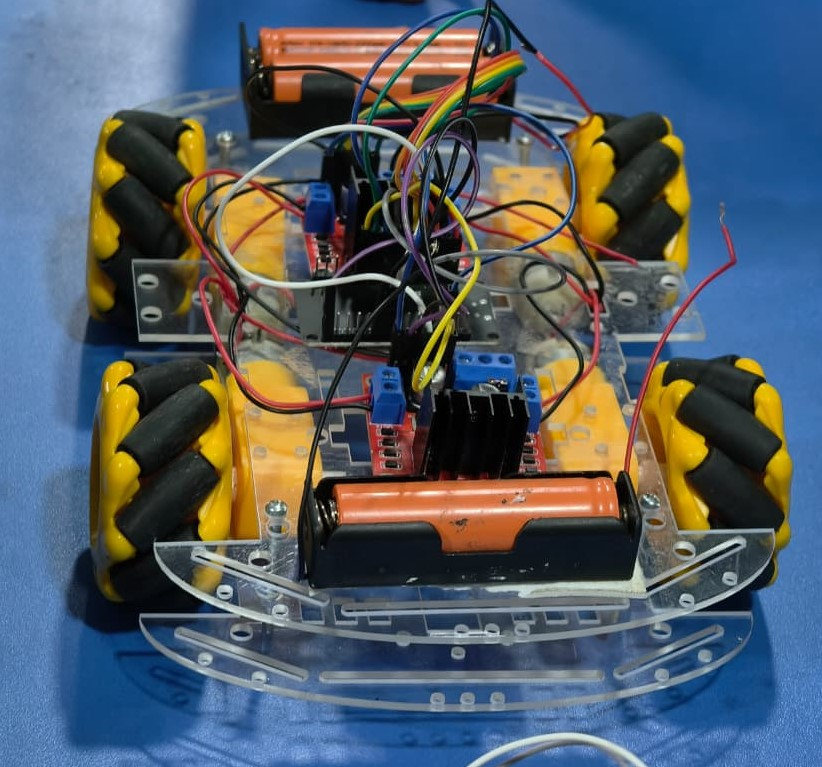
\includegraphics[width=\textwidth,height=6.5cm,keepaspectratio=true]{images/img1.jpeg}
  \captionof{figure}{Assembled 4WD Robot Car}
  \label{fig:assembled_car}
\end{minipage}
\hfill
\begin{minipage}{0.48\textwidth}
  \centering
  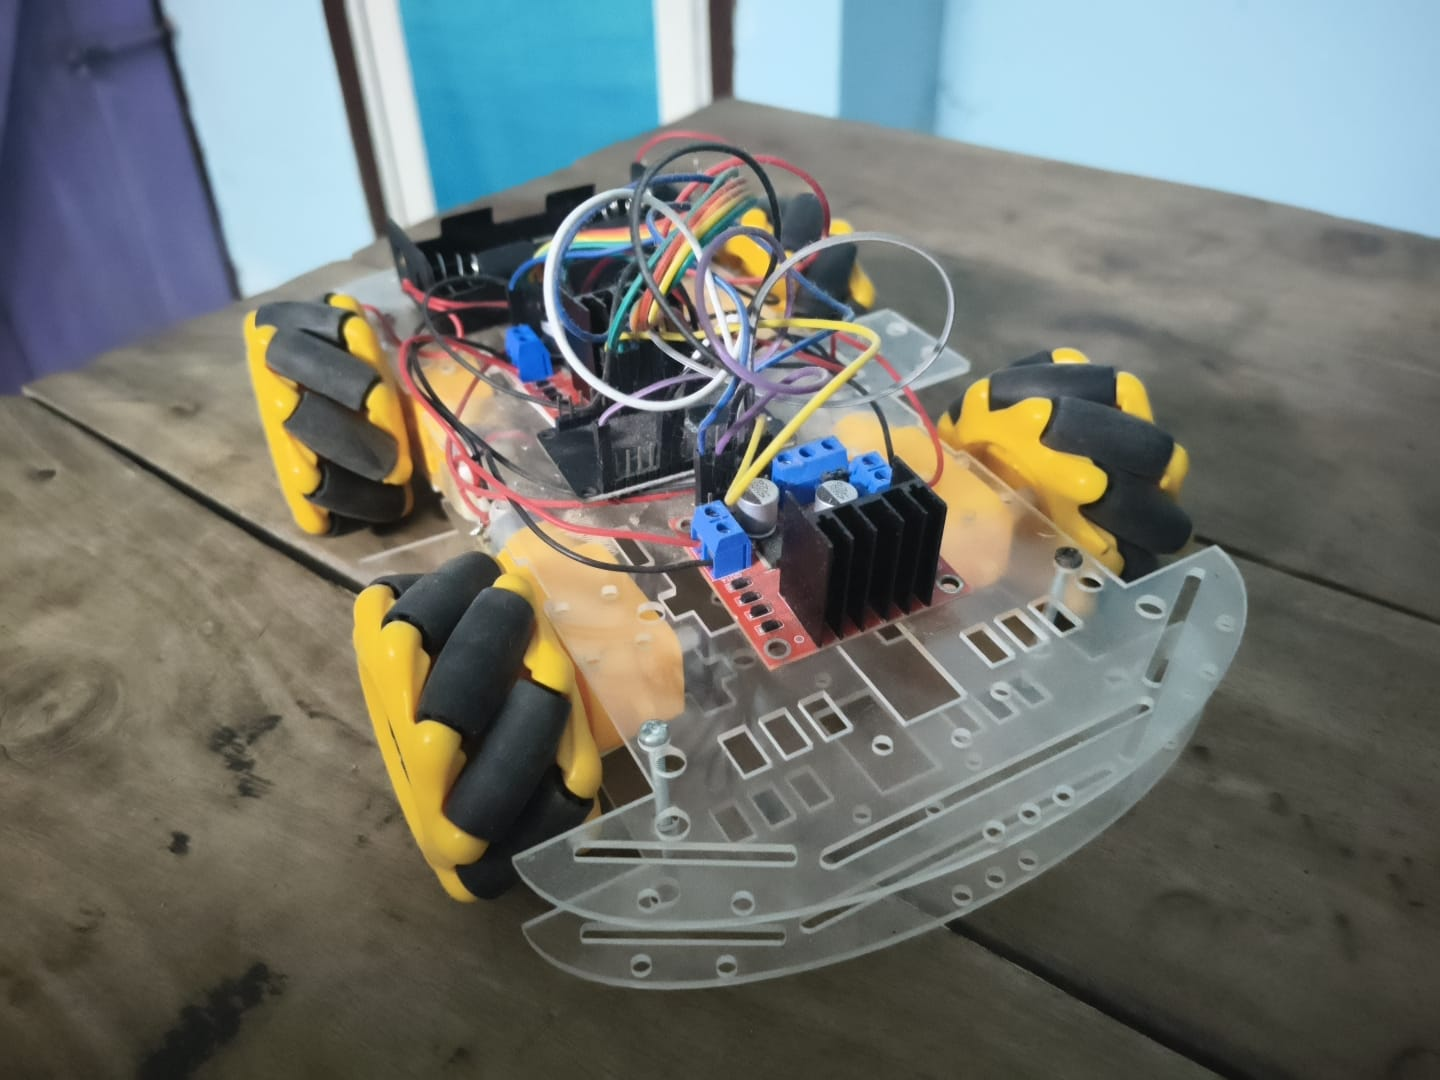
\includegraphics[width=\textwidth,height=6.5cm,keepaspectratio=true]{images/img2.jpeg}
  \captionof{figure}{Wearable Control Glove}
  \label{fig:glove}
\end{minipage}
\end{center}

\section{Performance Evaluation}
The prototype was evaluated on latency, range, and battery life. The ESP-NOW system achieved a latency of 8 ms and a reliable range of 45 m. A 2200 mAh 18650 battery pack provides 45 minutes of continuous operation. Figures \ref{fig:wiring}, \ref{fig:test}, and \ref{fig:battery} show the wiring, test, and battery mount setup.\par
\vspace{0.1in}
\begin{center}
\begin{minipage}{0.31\textwidth}
  \centering
  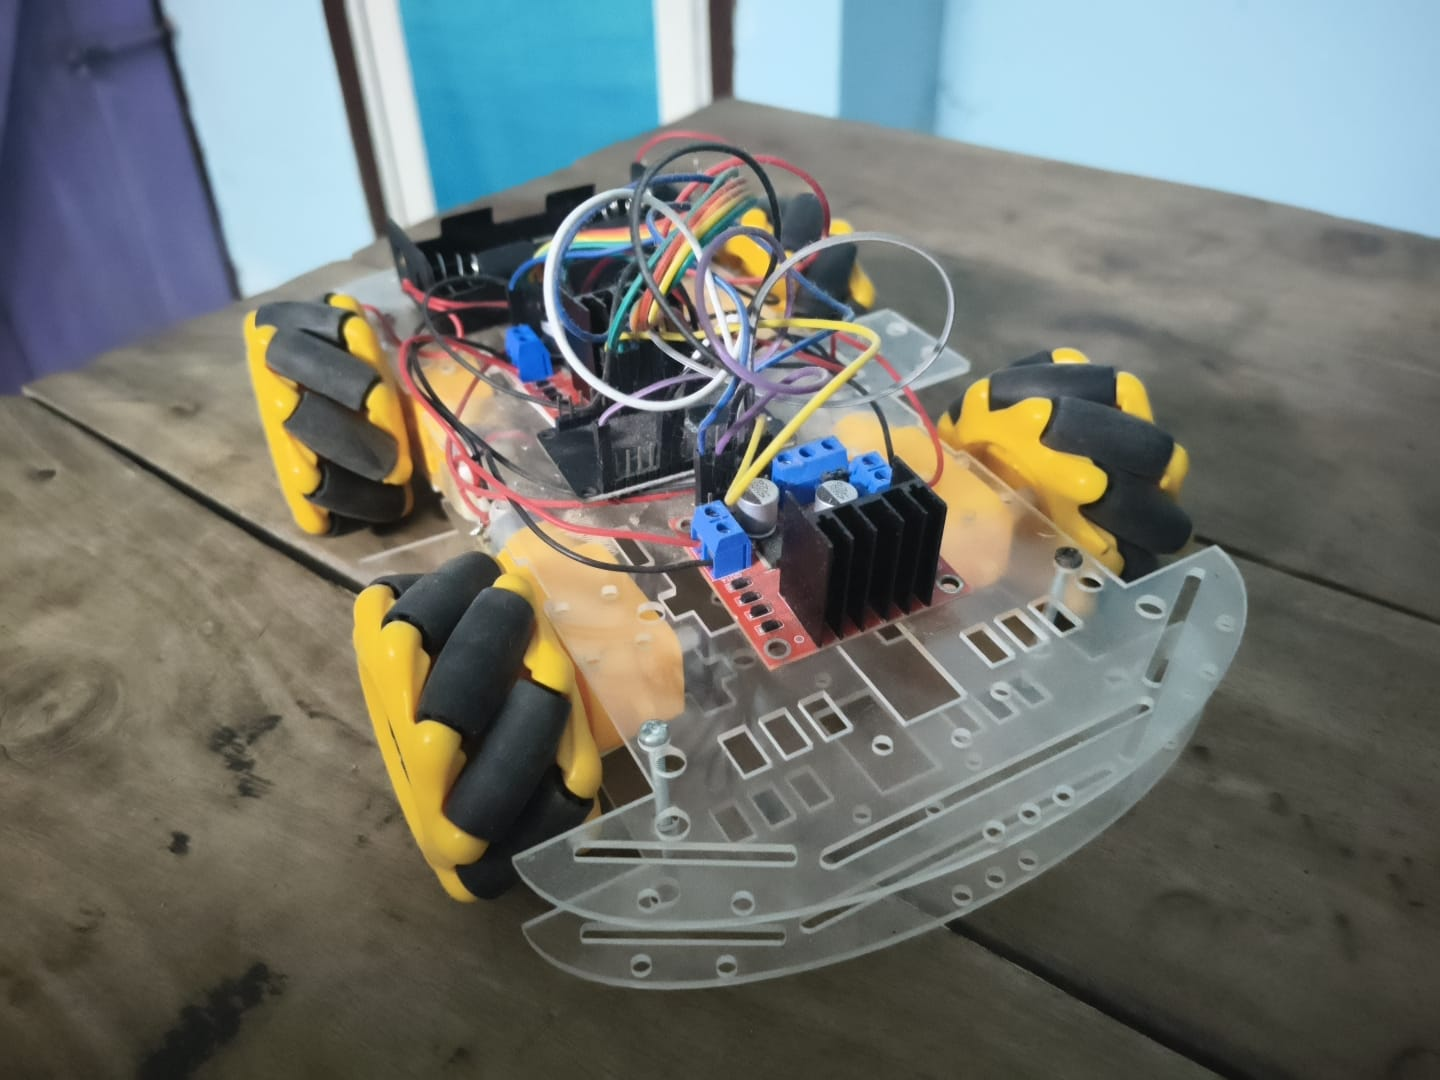
\includegraphics[width=\textwidth,height=5.5cm,keepaspectratio=true]{images/img3.jpeg}
  \captionof{figure}{Wiring Details}
  \label{fig:wiring}
\end{minipage}
\hfill
\begin{minipage}{0.31\textwidth}
  \centering
  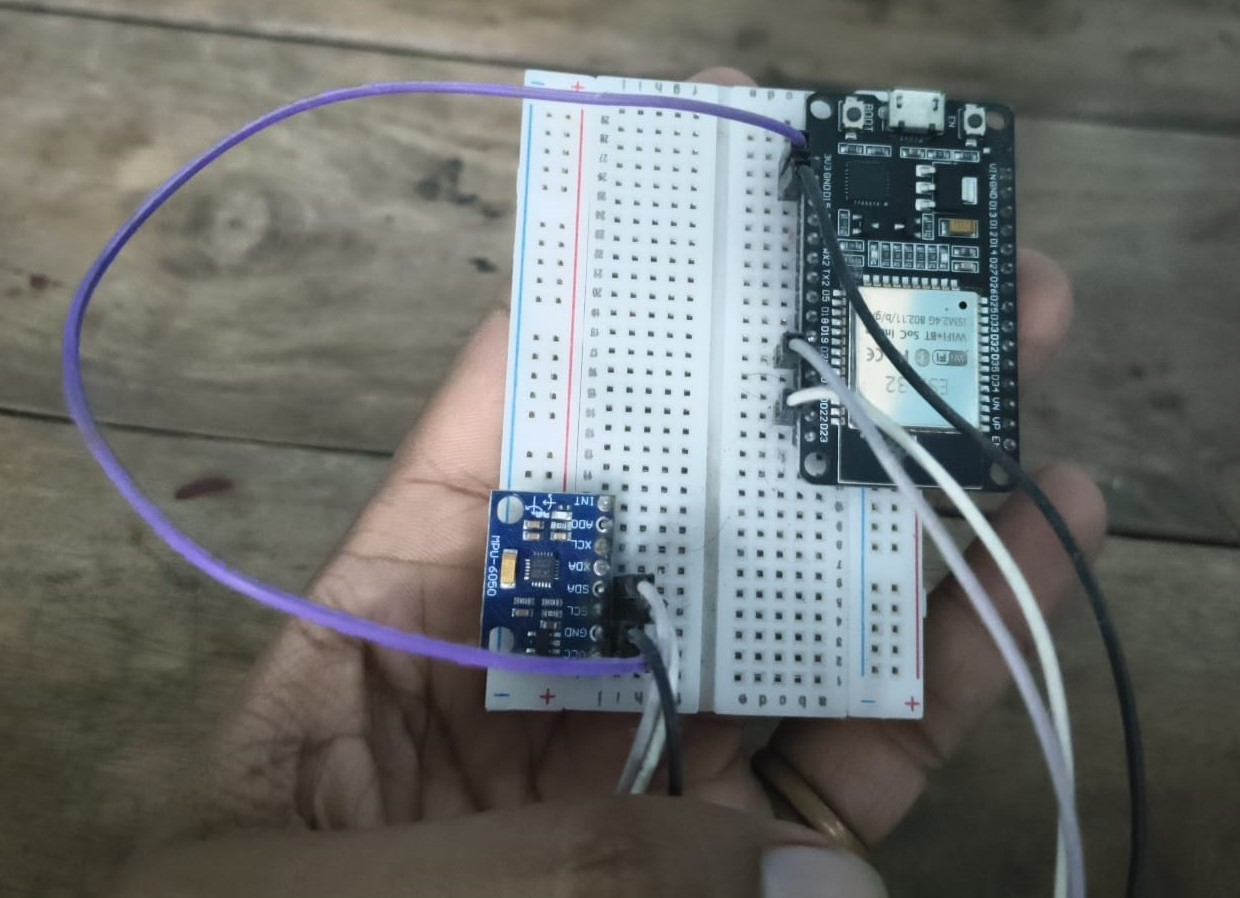
\includegraphics[width=\textwidth,height=5.5cm,keepaspectratio=true]{images/img4.jpeg}
  \captionof{figure}{Circuit Test}
  \label{fig:test}
\end{minipage}
\hfill
\begin{minipage}{0.31\textwidth}
  \centering
  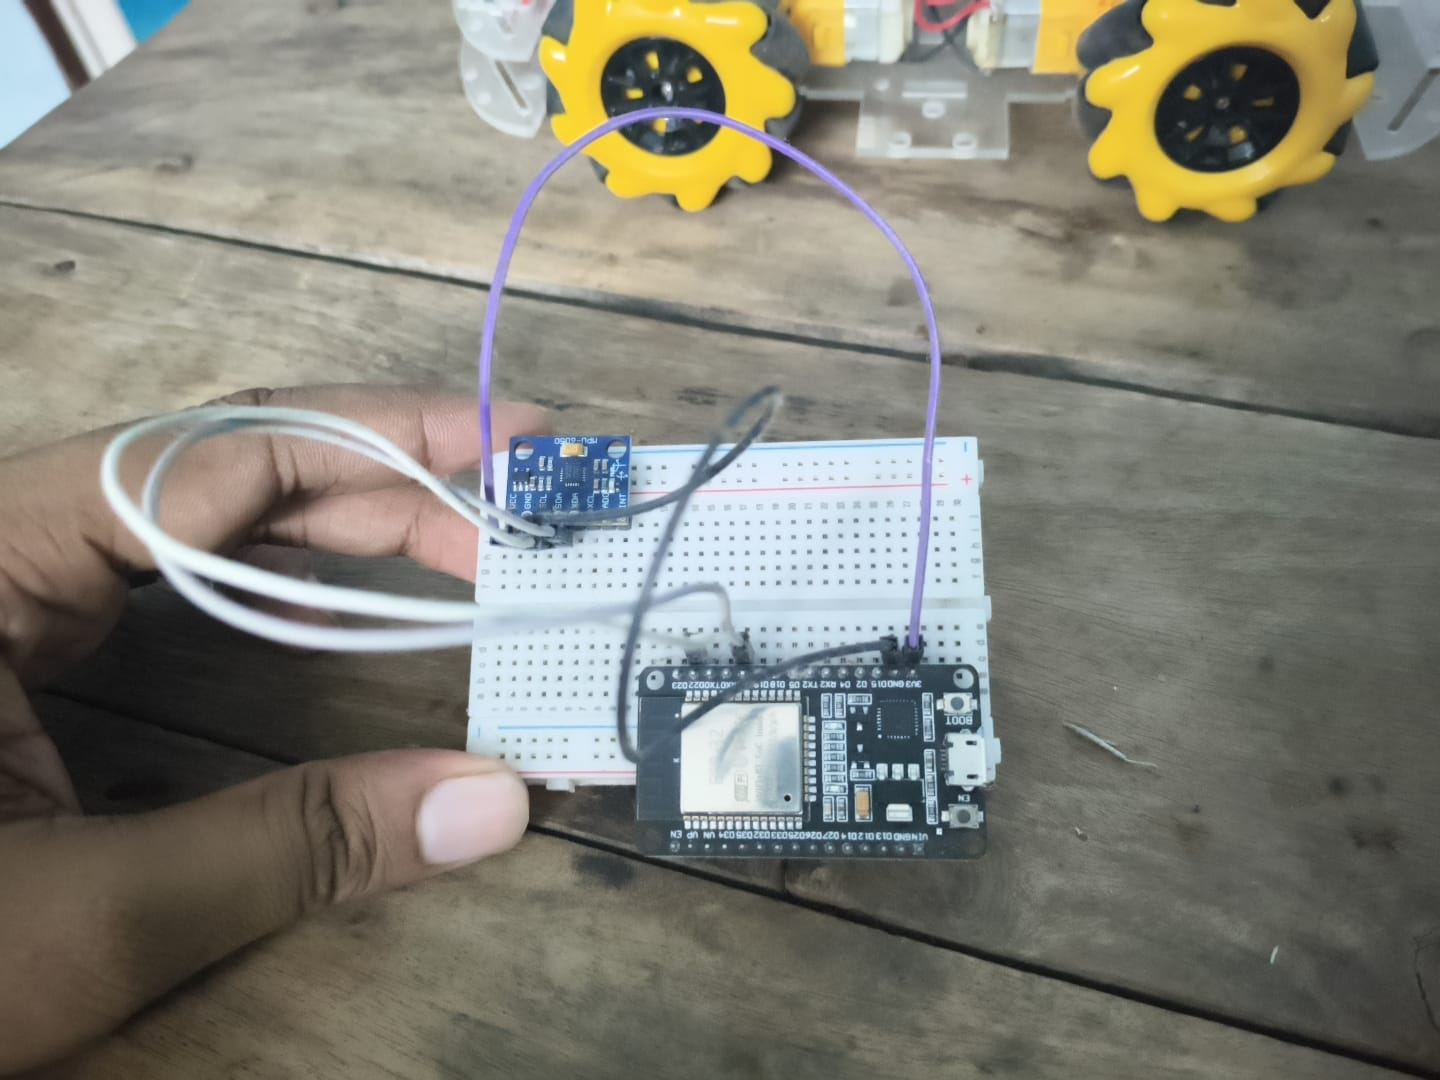
\includegraphics[width=\textwidth,height=5.5cm,keepaspectratio=true]{images/img5.jpeg}
  \captionof{figure}{Battery Mount}
  \label{fig:battery}
\end{minipage}
\end{center}

\section{Conclusions}
This mini project successfully demonstrates the design, construction, and physical calibration of an ESP32-based gesture-controlled 4WD robotic car. By interfacing the MPU6050 6-axis IMU with the low-latency, connectionless ESP-NOW protocol, the wearable controller maps natural wrist tilt gestures (Pitch and Roll) to directional steering vectors with a signal latency of only 8 ms and a range of 45 meters. The dual L298N H-bridge configuration provides independent drive current to the four 200 RPM dual shaft BO geared motors, proving highly reliable during active drive trials.\par
\medskip
In summary, the gesture-based interface offers a natural, hands-free alternative to traditional joysticks, making it highly accessible. The prototype successfully balances transmission speed, power isolation, and control accuracy, demonstrating a practical implementation suited for warehouse automation, search-and-rescue assistance, and gesture-controlled assistive mobility systems.

\section{Future Scope}
Future work includes replacing the L298N driver with the TB6612FNG, adding ultrasonic sensors for obstacle avoidance, implementing Kalman filters and sensor fusion algorithms for precise orientation tracking \cite{fusion_ref}, and integrating ROS for autonomous navigation in warehouse environments.

\clearpage
\begin{singlespace}
\begin{thebibliography}{99}
\addcontentsline{toc}{chapter}{References}
\setstretch{1.1}
\fontsize{10}{12}\selectfont
\setlength{\itemsep}{4pt}
\setlength{\parsep}{0pt}

\bibitem{sensor1}
A. R. Al-Ali and M. Al-Rousan, ``Java-Based Home Automation System,'' \textit{IEEE Trans. Consum. Electron.}, vol. 50, no. 2, pp. 495--501, 2004. DOI: 10.1109/TCE.2004.1309869.

\bibitem{imu_main}
InvenSense Inc., ``MPU-6000 and MPU-6050 Product Specification,'' Document Revision 3.4, Aug. 2013. Website: https://invensense.tdk.com/wp-content/uploads/2015/02/MPU-6000-Datasheet1.pdf.

\bibitem{espnow_ref}
Espressif Systems, ``ESP-NOW User Guide,'' ESP-NOW Technical Reference, 2021. Website: https://docs.espressif.com/projects/esp-idf/en/latest/esp32/api-reference/network/esp\_now.html.

\bibitem{motor_ref}
STMicroelectronics, ``L298 Dual Full-Bridge Driver Datasheet,'' SGS-THOMSON Microelectronics, Jan. 2000. Website: https://www.st.com/resource/en/datasheet/l298.pdf.

\bibitem{hmi_ref}
M. A. Al-Khedher, ``Wrist Hand Gesture Controlled Car Using Accelerometer Sensor,'' \textit{Int. J. Interact. Mobile Technol.}, vol. 7, no. 4, pp. 35--41, Oct. 2013. DOI: 10.3991/ijim.v7i4.3218.

\bibitem{robotics_ref}
J. J. Craig, \textit{Introduction to Robotics: Mechanics and Control}, 3rd ed., Upper Saddle River, NJ: Pearson, 2005. ISBN: 0201543613.

\bibitem{imu_filter}
J. K. John, ``Complementary Filtering of Gyroscope and Accelerometer Data for Gesture Recognition,'' \textit{Int. J. Embedded Syst.}, vol. 10, no. 2, pp. 115--122, 2018. DOI: 10.1504/IJES.2018.090604.

\bibitem{fusion_ref}
A. Gupta, ``MEMS Sensor Fusion Algorithms for Real-Time Orientation Estimation,'' \textit{IEEE Sensors J.}, vol. 19, no. 14, pp. 5612--5620, 2019. DOI: 10.1109/JSEN.2019.2905612.

\end{thebibliography}
\end{singlespace}

\end{document}
